\documentclass[final-report]{report-template}

\usepackage{graphicx}
\usepackage{amsmath}
\usepackage{tikz}
\usetikzlibrary{arrows.meta, positioning, shapes.geometric}

\graphicspath{{./figures/}}

\university{Imperial College London}
\department{Department of Earth Science and Engineering}
\course{MSc in Applied Computational Science and Engineering}
\title{Current Content Discovery for Module Teaching}
\author{Guanyuming He}
\email{guanyuming.he24@imperial.ac.uk}
\githubusername{esemsc-gh124}
\supervisors{Sean O'Grady\\
             Rhodri Nelson}
\repository{https://github.com/ese-ada-lovelace-2024/irp-gh124}

\newcommand\casemethod{case method}

\begin{document}

\maketitlepage  

\section*{Abstract}
TBD.
\textbf{Keywords:} content discovery, information retrieval, LLM, search engines, \casemethod, Business school,

\section{Introduction}
\subsection{Problem background}
Since the emergence of the first Business schools in the late 19th century
\cite{first.bis.school.1, first.bis.school.2}, several distinct pedagogical
teaching strategies have been applied.  First institutionalized at Harvard
Business School \cite{case.method.origin.1, case.method.origin.2} in the early
20th century, a method about teaching students with real world business cases
(will be called \emph{\casemethod} in the rest of the thesis) has been found
more effective and engaging \cite{case.method.support.1, case.method.support.2,
case.method.support.3} than many traditional, for example, big lecture based,
teaching methods. The \casemethod\ is valued as a form of \emph{active
learning} methods for students, for its ability to expose students to complex,
context-specific problems that lack clear-cut solutions. As such, it has found
wide adoption across the world \cite{case.method.adoption.1,
case.method.adoption.2}.

However, despite its aforementioned adoption and performance in business school
teaching, the case method faces a significant constraint: the availability and
collection of timely and relevant case material \cite{case.method.limit.1,
case.method.limit.3}. In particular, Christensen has identified in his classical
article that instructors would have to conduct ``extensive preparation''
\cite{case.method.limit.2} for case method. Another factor contributing to this
constraint of case method is the ever-evolving business world and the necessity
of the latest information: Clark argues that, because learned skill will lose
value quickly in five years, it is critical for students to be up to date to
remain relevant in the business world \cite{case.method.limit.4}; McFarlane
emphasises the importance of updated cases, as otherwise students could be
disengaged or discouraged \cite{case.method.limit.5}.

\subsection{Past advancements in information retrieval}
During the past two centuries, a number of key developments have profoundly
expanded an individual's capacity to retrieve information about the world. In
the early 19th century, the transmission of information was still traditional
--- carried by person on paper or simply remembered. This fundamentally limited
both the speed and geographic reach of information retrieval. The invention of
telegraph in the 1840s by Morse, Cornell, and Henry \cite{history.telegraph.1,
history.telegraph.2}, notably with Morse's first telegraph message,
``\emph{What hath God wrought?}'' in 1844 \cite{first.telegraph.msg}, marked a
paradigm shift by enabling very fast transmission of encoded information over
relatively short distances (w.r.t.\ the earth) via wired networks.  This
technological innovation was considerably improved by the invention of the
telephone by Bell in 1876 \cite{history.telephone.1, history.telephone.2},
enabling communication directly by human voice, instead of encoded Morse code.

Wired communication is critically constrianed by geographical
features on where the wires were laid. Around the late 19th century, 
Marconi's experiments with wireless telegraphy \cite{history.wireless.1} and
the first successful transatlantic signal in 1901
\cite{history.first.atlantic.broadcast} introduced electromagnetic wave-based
wireless communication, eventually accumulating into the world's first voice
broadcast by radio in 1906 \cite{first.voice.broadcast}. These milestones
collectively redefined the temporal and spatial boundaries of information
access.

The next many decades have seen people improving on the serious limitations of
wireless communication: signal strength, interferences and attenuation,
carrying capacity, and even deliberate sabotage during war times
\cite{wireless.weakness.1, wireless.weakness.2, wireless.weakness.3}.
Theoretically, Hartley observed a logritham pattern of information capacity
\cite{hartley.log.information} and then Shannon expanded on it to first define
\emph{bits} and \emph{entropy}, giving a formal mathematical theory of
information \cite{shannon.theory.communication} in 1948. Meanwhile,
engineers were experimenting with alternative modulation techniques, notably
frequency modulation (FM), and the concepts were formalized in the 1930s
\cite{history.modulation}. 

As the theoretical understanding of information progressed, people began to
have the idea of \emph{searching} for information based on content
and by relevance, instead of by unique identifier
\cite{history.information.retrieval}. Actually, the term \emph{information
retrieval} was not invented until Mooers coined it in 1950
\cite{mooers.info.ret.term}. Since then, information retrieval systems have
quickly evolved, and went through four phases before 2000: ``(1) manual and mechanical
devices; (2) offline computing; (3) online computing, vendor access; (4)
distributed, networked, and mass computing.'' \cite{info.ret.4.phases}, with
the last three substantially contributed to by the invention of the Internet
\cite{history.internet}, and consequently the emergence of search engines in
the 1990s \cite{history.search.engines, history.internet.search.engines}.
For the next two decades, search engines greatly expanded in speed and
coverage and has been significantly impacting the society's information for at
least a decade \cite{search.engine.impact.1, search.engine.impact.2}.
Nevertheless, one would need to carefully craft search engine prompts into
clearly and precise list of words or a short sentence, often necessitating the
use of advanced search features, such as boolean query (i.e. use logical
connections like \texttt{AND}, \texttt{OR}) to achieve desired performance
\cite{advanced.search.necessity.1, advanced.search.necessity.2}.


LLMs have undoubtedly entered and transformed many areas, including daily life,
business and the industry, and research \cite{llm.impact.1}. One strong appeal
of LLMs is that they could process user's natural language input and generate
natural language output in return with remarkable resemblence to what a human
would say \cite{llm.power.1, llm.power.2}. However, because of the inherent
limit of neural networks, some argue that they could not formally reason about
what they output \cite{llm.limit.1, llm.limit.2, llm.limit.3}. Indeed,
hallucination \cite{llm.hallucination.1, llm.hallucination.2} and other forms
of distortion of facts, is a big problem of LLMs. On the other hand, although
search engines rely on determinstic algorithms that give precise reference to
searched result, they could not compare with LLMs' ability to process search
prompts and summarize results. 

Therefore, various attempts have been made to integrate LLMs with search
engines \cite{llm.meet.search.1, llm.meet.search.2, llm.meet.search.3}.
Specifically, Xiong et al.\ proposes to categorize them into ``LLM4Search'' and
``Search4LLM'', where ``A4B`` means using A to improve B
\cite{llm.meet.search.1}. Here is where my thesis will build upon.  Now, with
the help with LLMs that can easily process frivolous natural language input, I
plan to integrate them together to boost information retrieval further,
especially in the area of business school teaching content discovery.

To summarize the above overview of the history,
\begin{itemize}
	\item Information retrieval had been a manual, incomplete, and slow process
		for many centuries.
	\item Technical inventions and theoretical advancements in the 19th and
		20th centuries improved on all of the aspects, greatly increasing the
		reach and speed of the spread of information.
	\item The invention of digital computers had transformed the manual labor
		of searching for and filtering information into a semi-automatic
		manner. Additionally, the Internet has connected the previously
		separated information storages around the world.
	\item Still, current search engines operate semi-automatically, requiring
		careful craft of search prompts. On the other hand, LLMs allow for
		frivolous prompts but often hallucinates.
\end{itemize}

\subsection{Goals}
In this project, I will attempt to improve the current state of information
retrieval (mostly limited to business teach related information) further by
designing and developing a software
system. More precisely, these are the goals:
\begin{enumerate}
	\item By combining LLMs and search engines, compensate each other's
		weakeness in information retrieval.
		\begin{enumerate}
		\item The system shall improve search engines on prompt engineering to
			the extent that a user would only need to give a rough and vague
			natural language description of the target information to the
			system.
		\item The system shall improve LLMs on result credibility and
			interpretibility. If pure LLMs lack the two properties, then
			combination with deterministic and well-designed ranking and
			searching algorithms in search engines will compensate for that.
		\end{enumerate}
	\item Enhance the automation of the current general public information
		retrieval tools, e.g., Google search, ChatGPT, to the extent that a
		user would only need to occasionally configure the system, instead of
		giving search prompts each time.
	\item Specially tailor the system to business teaching related information,
		aiming to gather information from authentic and reliable sources.
	\item The system shall support up-to-date information retrieval. More
		precisely, the system shall support the user to specify a time range of
		information, and the user is allowed to set the end of the range to the
		current time.
	\item The system could support user feedback and learning from it to
		provide information more close to one's need.
\end{enumerate}

\subsubsection{Not included in the goals}
On the other hand, these possible targets are beyond the scope of my project:
\begin{enumerate}
	\item Providing a method to rank business information. This is rather
		subjective and I believe is better left for the user to judge.
	\item Enforcing strict security measures. Because the use group of the
		system is limited to business school teaching teams, enforcing output
		security or censorship of harmful or adult content is not a goal.
\end{enumerate}

\section{Methods} 
\subsection{Architecture}
Based on the goals, the system is designed to be a chain of tools invoking each
other.

What directs the system is the user's configuration, which is expected to
include
\begin{enumerate}
	\item A time range of information to retrieve.
	\item A natural language description of the types of information to
		retrieve.
	\item How the retrieved information is sent to the user.
	\item A frequency of running the tool.
\end{enumerate}

Based on the configured running frequency, the tool runs, which
\begin{enumerate}
	\item Use LLMs to translate the configured description and generate a list
		of search engine prompts.
	\item The prompts are fed to search engines, with the configured time
		constraint.
	\item The search results are gathered and processed. How the information is
		processed and filtered may rely on other AI systems like a
		rule-based expert system.
	\item The processed results may be summarized by LLMs.
	\item The results are sent to the users via the configured ways.
	\item Optionally, the user gives feedback to the results. The tool can
		thus improve on the search engine prompts, the information processing,
		and LLM parameters, based on the feedback. The improvement algorithm
		may use something like recommendation algorithms. Then, the tool can
		iterate on the user's configuration automatically.
\end{enumerate}

Figure~\ref{fig.arch.flow} demonstrates my architecture design and the workflow
of the system.

\begin{figure}[htbp]
\centering
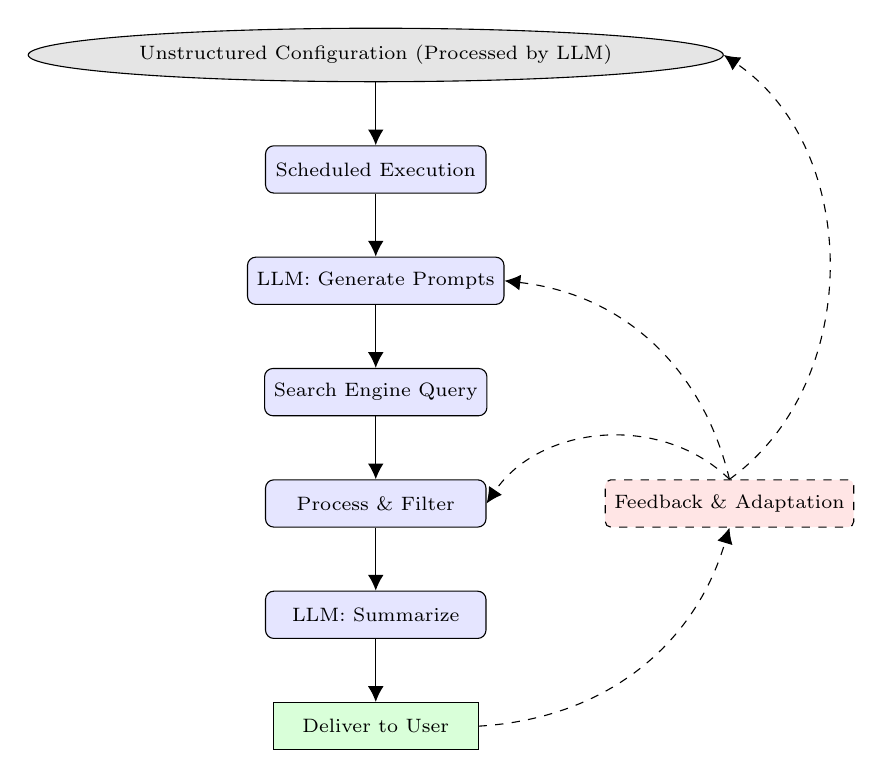
\begin{tikzpicture}[
	  node distance=0.8cm,
  every node/.style={font=\scriptsize},
  process/.style={draw, rounded corners=3pt, fill=blue!10, minimum width=2.8cm, minimum height=0.6cm, text centered},
  input/.style={draw, ellipse, fill=gray!20, minimum width=2.6cm, minimum height=0.6cm},
  output/.style={draw, rectangle, fill=green!15, minimum width=2.6cm, minimum height=0.6cm},
  feedback/.style={draw, dashed, fill=red!10, rounded corners=2pt, minimum width=2.6cm, minimum height=0.6cm},
  arrow/.style={-{Latex[width=2mm,length=2mm]}, line width=0.5pt},
  fb/.style={-{Latex[width=2mm,length=2mm]}, line width=0.4pt, dashed, bend right=35}
]

% Main vertical flow
\node[input] (config) {Unstructured Configuration (Processed by LLM)};
\node[process, below=of config] (scheduler) {Scheduled Execution};
\node[process, below=of scheduler] (promptgen) {LLM: Generate Prompts};
\node[process, below=of promptgen] (search) {Search Engine Query};
\node[process, below=of search] (processresults) {Process \& Filter};
\node[process, below=of processresults] (summarize) {LLM: Summarize};
\node[output, below=of summarize] (deliver) {Deliver to User};
\node[feedback, right=1.5cm of processresults] (feedback) {Feedback \& Adaptation};

% Arrows (main flow)
\draw[arrow] (config) -- (scheduler);
\draw[arrow] (scheduler) -- (promptgen);
\draw[arrow] (promptgen) -- (search);
\draw[arrow] (search) -- (processresults);
\draw[arrow] (processresults) -- (summarize);
\draw[arrow] (summarize) -- (deliver);

% Feedback arrows (clean curves)
\draw[fb] (deliver.east) to (feedback.south);
\draw[fb] (feedback.north) to (promptgen.east);
\draw[fb] (feedback.north) to [bend right=50] (processresults.east);
\draw[fb] (feedback.north) to [bend right=55] (config.east);
\end{tikzpicture}
\caption{Architecture and operational flow of the software system}
\label{fig.arch.flow}
\end{figure} 	

What directs the system is the user's configuration, which is expected to
include a time range of information to retrieve, a natural language description
of the types of information to retrieve, how the retrieved information is sent
to the user, and a frequency of running the tool.

\subsection{Implementation plan}
In this section, I give the plan of my implementation. It is for the project
plan and only has specific directions, not concrete programming language, tool,
or frameworks, as they will subject to tests and changes during the project.
In the thesis, I will replace them with details.

\subsubsection{Configuration format} 
LLMs have demonstrated unprecedented ability to process unstructured data
\cite{llm.unstructured.data.1, llm.unstructured.data.2}. Thus, it is desirable
for the system to accept unstructured configuration from the user. The user may
give a natural language description of the wanted information, give some
examples, e.g., URLs, or simply feed the LLM the teaching slides and videos
from previous classes.

Nevertheless, there are a few configurations that must be formatted.
\begin{enumerate}
	\item A range of time for the information retrieved.
	\item (Optional) A list of sources (e.g. websites) to always include or exclude.
	\item The destination of the collected information (e.g. email addresses of
		teaching staff).
\end{enumerate}
Of course, LLMs can still try to infer them from the given unstructured data,
but they must be presented to the user for her to decide and correct, because
these configurations are strict and a little error will have great effects.

Another important output from unstructured configuration is the search prompts
or insturctions generated by the LLMs. As this output direct controls the
information retrieved. LLMs for this task will be specifically tuned to ensure
\begin{itemize}
	\item Diversity of results.
	\item A specific distribution of results. E.g., a more authentic website
		will contribute relatively more information.
\end{itemize}

\subsubsection{Scheduled Execution} Based on the configured running frequency,
the system will run every once a while automatically. The scheduling component must handle
different frequencies (daily, weekly, monthly) and manage execution timing to
avoid overwhelming external APIs or generating excessive costs. This involves
implementing a robust scheduling system that can handle failures, retries, and
load balancing across multiple users.

\subsubsection{Multi-Source Search Integration} 
One problem of search engine APIs is that they have ungenerous search limits
\cite{search.api.limit.1}, allowing about 1000 queries per month, which is not
enough for frequent testing and prototyping.

As a result, I plan to use some other self-developed system in parallel with
search engines, which do only a small amount of tasks that truly require whole
Internet searching. The majority of the searching will be handled by scraping a
limited sets of websites, most likely.

\subsubsection{Content Processing and Filtering} Search results will be
gathered and processed through a multi-stage filtering system. This involves
content deduplication, relevance scoring, source credibility assessment, and
quality filtering. The processing pipeline will need to handle various content
formats including articles, reports, videos, and social media posts.

The filtering system will combine rule-based approaches (such as keyword
matching and source whitelisting) with machine learning techniques for
relevance scoring and content classification. Natural language processing
techniques will be employed to extract key information and assess content
quality. The system will also need to handle different languages and cultural
contexts in business information.

\subsubsection{LLM-Based Summarization} Processed results will be summarized
using LLMs with business-focused prompting strategies. The summarization
component must balance comprehensiveness with conciseness, ensuring that key
business insights are preserved while making information digestible for
educators. This involves developing prompting strategies that can identify the
most relevant information for case method teaching and present it in a
structured format.

The summarization process may involve extractive techniques (selecting key
sentences from original content) and abstractive techniques (generating new
summaries). Different summarization styles may be needed for different types of
content and user preferences.

\subsubsection{Delivery and User Interface} Results shall be sent to users via
configured methods, which may include email summaries, web dashboards, or
integration with existing educational platforms. The delivery component shall
handle different user preferences and ensure information is presented in a
format suitable for educational use.

\subsubsection{Feedback and Adaptation System} The system shall collect user
feedback on result quality and relevance, using this information to improve
future searches. This involves designing feedback mechanisms that capture both
explicit user ratings and implicit behavioral signals. Possible algorithms
include recommendation algorithms and other machine learning models.

\subsection{Technical Considerations} 
The system will be a high-level program, which calls for simply programming
languages like Python. On the other hand, the system may have specific
performance requirements, especially for LLMs and other machine learning
algorithms. The likely result is a combination of different programming
languages and technical frameworks.

\subsection{Evaluation and Validation} System effectiveness will be evaluated
through multiple metrics including information retrieval precision and recall,
user satisfaction surveys, time savings measurements, and comparison with
manual search processes. Evaluation will involve collaboration with business
educators to assess the practical utility of discovered content for case method
teaching.

The system will be tested with different types of business information requests
and across different time periods to ensure robust performance. A/B testing may
be employed to compare different algorithmic approaches and user interface
designs.


\section{Results}

\section{Discussion}

\section{Conclusion}

\clearpage

% References
\bibliographystyle{plain}
\bibliography{references.bib}  % BibTeX references are saved in references.bib

\end{document}          
